% boidherd: the project report for Intelligent Robotic Systems.
% Build: tectonic main.tex  (from this folder; figures come from tools/analyse.py)
\documentclass[11pt,a4paper]{article}

\usepackage[margin=2.5cm]{geometry}
\usepackage{fontspec}             % Tectonic is XeLaTeX
\usepackage{amsmath,amssymb}
\usepackage{graphicx}
\usepackage{booktabs,array}
\usepackage{subcaption}
\usepackage{xcolor}
\usepackage[round,authoryear]{natbib}
\usepackage{qrcode}
\usepackage{tikz}
\usetikzlibrary{positioning,arrows.meta}
\usepackage[hidelinks]{hyperref}
\usepackage[nameinlink]{cleveref}

\graphicspath{{figures/}}

% A video in a PDF won't play in most viewers: a still frame that links to it,
% with a QR code for the printed page.
% \videofigure{frame image}{url}{caption}{label}
\newcommand{\videofigure}[4]{%
  \begin{figure}[tbp]
    \centering
    \begin{minipage}[c]{0.78\linewidth}
      \href{#2}{\includegraphics[width=\linewidth]{#1}}
    \end{minipage}\hfill
    \begin{minipage}[c]{0.18\linewidth}
      \centering\qrcode[height=2.2cm]{#2}
    \end{minipage}
    \caption{#3 Video: \url{#2}}
    \label{#4}
  \end{figure}}

% Notes to self while drafting; empty this to hide them.
\newcommand{\todo}[1]{\textcolor{red}{[#1]}}

\title{Leading a drone flock past a dead end:\\
  three flocking models and a planning layer for informed leaders}
\author{Marco Galeri\\
  \small Intelligent Robotic Systems, Alma Mater Studiorum -- Università di Bologna}
\date{November 2026}

\begin{document}
\maketitle

\begin{abstract}
  A few informed leaders, which the others cannot recognise, have to bring a
  flock of simulated Crazyflie drones to a goal only they know. Three flocking
  models, Reynolds' boids, Couzin's zone model and a hybrid built on
  Vásárhelyi's model for real drones, fly on the same robot, with the same
  leaders, behind one interface; the leaders can add a deliberative layer
  that plans a path on the known map and follows it. On maps none of the
  models was tuned on, 450 runs paired by starting position show that the
  planner is what gets Reynolds' flock past a corner or a dead end at all, that
  more leaders help as Couzin predicted only in Couzin's model, and that the
  hybrid fails with two leaders that plan different ways round an obstacle:
  its flock follows their average, into the obstacle. What a model makes a
  follower do, cruise on its own, wait to be pulled, or keep a direction to be
  outvoted, explains each model's strengths and failures; no flock reached the
  goal without leaders.
\end{abstract}

\section{Introduction}
\label{sec:introduction}

% The task, in a paragraph: n Crazyflie drones flock from sector A to sector C
% of a known map; only j of them (the informed leaders) know where C is, and
% nothing marks them to the others (Couzin 2005). Design log: 2026-10-14
% "Research question".
\todo{The task.}

% Why it is interesting: leadership without recognition in a flock; a
% reactive swarm meets obstacles a reactive leader can't solve (a dead end).

% The questions, as stated hypotheses (slides 1.3: state them before the
% experiments). Draft:
%   H1  Without leaders no flock reaches C within the time a guided flock
%       needs (the j = 0 control).
%   H2  More leaders bring the flock more reliably (Couzin et al. 2005).
%   H3  A planning layer for the leaders is needed where steering straight
%       at C leads into a dead end.
%   H4  The three flocking models differ in how well their followers follow.
\todo{Hypotheses H1--H4.}

% What the project contributes, and the report's structure (one line per
% section).
\todo{Contributions and outline.}

\section{State of the art}
\label{sec:background}

\subsection{Swarm robotics}

Swarm robotics designs the collective behaviour of many simple robots that
act on local sensing and communication, without central control
\citep{brambilla2013}. Brambilla et al.\ classify the behaviours studied into
spatial organisation (aggregation, patterns), navigation (collective
exploration, coordinated motion, collective transport) and collective
decision making, and the design methods into behaviour-based design, by hand,
and automatic design. This project is a case of coordinated motion, flocking,
that carries a collective decision, where to go, made by a few informed
members; its controllers are designed by hand and studied in simulation.

\subsection{Flocking models}

\citet{reynolds1987} produced flocks for computer animation from three local
rules, each an acceleration: separation from neighbours that are too close,
alignment with their velocity, and cohesion toward their centre. Boids see
perfectly and respond at once, and they remain the usual starting point for
flocking robots: \citet{hauert2011} flew Reynolds' rules with a migration
point on ten fixed-wing robots, noting that a rotorcraft, which can move in
any direction, is the easiest robot to fly them on.

\citet{couzin2002} cast the same ingredients as zones around an individual: it
moves away from neighbours in the zone of repulsion, and only if there are
none, aligns with those in the zone of orientation and moves toward those in
the zone of attraction. Changing the widths of the zones makes a group switch
between a swarm, a milling torus and a parallel group, and the group's
history decides which, a collective memory.

\citet{olfatisaber2006} gave flocking a theory for agents with inertia: the
free rules generically break a flock into pieces, and a navigational
feedback, a virtual leader, holds it together and steers it; obstacles enter
as virtual agents.

Bringing the models to real flying robots meant modelling the robot.
\citet{viragh2014} describe a flying robot by its imperfections, the time it
takes to respond, its largest acceleration, delays, noise and limited range,
and show that delays make an ideal flocking model oscillate and collide; they
replace the stiff separation with a linear repulsion and add a pairwise
\emph{friction}, an alignment that damps velocity differences between close
neighbours. \citet{vasarhelyi2018} flew 30 drones with such a model in a
confined arena, its parameters optimised by evolution. Walls and obstacles
are virtual agents at their nearest point, flying away from them, with which
a drone aligns along a braking curve: the closer the wall, the less it may
fly toward it. Their arena has no goal: the flock only has to stay together
and inside.

Reactive models have limits in clutter. \citet{soria2021} show that the
potential-field family of swarm models does not guarantee fast and safe
flight among obstacles, and replace it with model predictive control.

\subsection{Leadership in groups on the move}

\citet{couzin2005} asked how animal groups move toward a goal that only a few
of their members know, when the others cannot tell who those are and nobody
signals. Their informed individuals are ordinary members of a zone-model
group, with one difference: they mix a preferred direction into the direction
their neighbours suggest, with a weight $\omega$. Three results frame this
project:
\begin{enumerate}
  \item a small informed minority can guide a large group, and the accuracy of
        the group grows with the fraction of informed individuals;
  \item the larger the group, the smaller the fraction needed for the same
        accuracy;
  \item with two informed subgroups preferring different directions, the
        group follows their average when the directions differ little, and
        chooses one of them, usually the larger subgroup's, when they differ
        a lot.
\end{enumerate}
The followers in this project are uninformed in the same sense: they don't
know where the goal is and can't recognise the leaders.

\subsection{Deliberative and hybrid control}

A purely reactive controller maps what a robot senses to what it does; a
deliberative one plans on a model of the world. Hybrid architectures put a
deliberative layer on top of a reactive one, which keeps the robot safe while
the plan gives it direction \citep{arkin1998}. Path finding on a grid with A*
\citep{hart1968}, with a cost that grows near obstacles, and path following by
pure pursuit, which steers toward a point a fixed distance ahead along the
path \citep{coulter1992}, are standard ways to fill the two layers in mobile
robotics. This project gives such a layer to the leaders only, on top of the
flocking model, and leaves the followers purely reactive.

\section{System overview}
\label{sec:system}

This section describes what was built and how the pieces fit together; the
flocking models and the leaders' planner, the parts the experiments compare,
are described in \cref{sec:controllers}. Every choice below was recorded when
it was made, with its reason and the alternatives turned down, in a design
log kept with the code (\texttt{docs/design-log.md}); the section summarises
it.

\subsection{Platform}
\label{sec:platform}

The project runs in Webots R2025a \citep{michel2004}, on its model of the
Bitcraze Crazyflie~2.1, a 10\,cm quadrotor \citep{giernacki2017}. Each drone
runs its own controller, written in Python~3.11; a supervisor, the
\emph{referee}, logs every drone's true position and velocity at every step
for the analysis and takes no part in the flight. The simulation step is
16\,ms.

\paragraph{Why a drone.} Reynolds' boids are point masses: each rule yields
an acceleration, and velocity and position follow from it. A wheeled robot
such as the e-puck, the course's usual robot, cannot behave like that: its
wheel speeds set its velocity directly, with no momentum, and it moves only
where it faces. A quadrotor has inertia and moves in any direction
whatever its heading, so it is the robot closest to a boid
\citep{hauert2011}; it is also the robot real drone flocks are built from
\citep{vasarhelyi2018}. Turned down: a ballbot or a spherical robot, where
balancing or steering would have become the project.

\paragraph{A drone with the real one's limits.} The Webots model is more
capable than the real Crazyflie, so two limits were added to keep the
controllers honest: the motors are capped so that the total thrust is about
twice the weight, as on a real Crazyflie~2.1 (the model's own limit gives over
a hundred times), and the commanded tilt is capped at 30\textdegree.

\paragraph{Flat flight.} All drones fly at one altitude, so the flock moves
in the plane and every obstacle blocks. The code is three-dimensional
throughout, with a single gain switching vertical motion on, but flying over
obstacles was left as future work (\cref{sec:conclusion}).

\subsection{Maps and worlds}
\label{sec:maps}

A map is a small TOML file that describes geometry only: the arena as a union
of axis-aligned rectangles, sector A (the spawn) and sector C (the goal) as
rectangles, and obstacles, walls as boxes and pillars as cylinders, placed by
hand or grown as a seeded forest. The number of drones~$n$, of leaders~$j$ and
the seed belong to the run, not to the map, so one map serves a whole
experiment. A world is generated in four steps, each a pure function tested
without Webots:
\begin{enumerate}
  \item \emph{load} the file into validated data classes (unknown keys are
        rejected with a suggestion, so a typo can't silently change a map);
  \item \emph{build} the course: the arena outline as wall boxes, the
        forests, and checks that need geometry, among them that C can be
        reached from A;
  \item \emph{spawn} the swarm with the run's seed: $n$ drones on the floor
        of A, at a constant density (2\,m$^2$ each, redrawn until they form
        one connected group), and $j$ of them chosen at random as leaders;
  \item \emph{render} the Webots world file.
\end{enumerate}
The obstacle layout has its own seed, in the map, so a change in results can
never come from a different course; the run's seed changes only where the
drones start and which of them lead.

\Cref{fig:maps} shows the three maps of the experiments. \texttt{l\_hall}, a
wide L-shaped hall with a pillar forest before the turn and a wall with a 4\,m
gap after it, is the map the models were developed and tuned on.
\texttt{l\_turn} is the same hall with nothing in it. \texttt{dead\_end} is an
open room with a cup between A and C, open toward A: the straight line from A
to C ends in its bottom, so a leader that steers straight at C leads its flock
into the cup.

\begin{figure}[tbp]
  \centering
  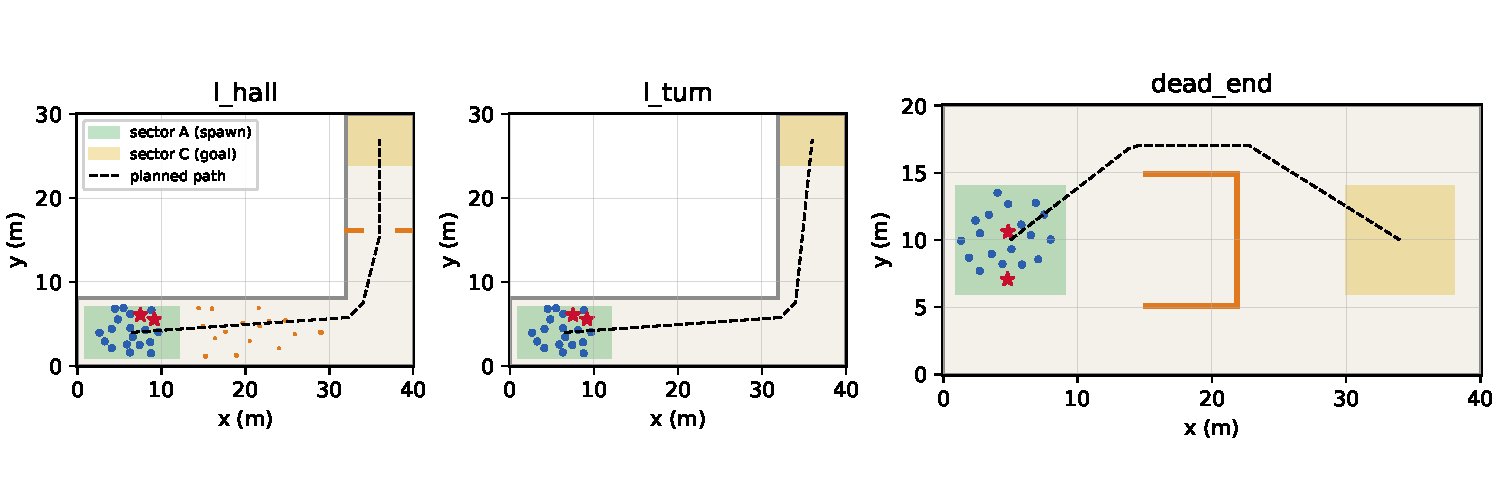
\includegraphics[width=\linewidth]{maps}
  \caption{The maps from above, each with a 20-drone spawn (seed~0):
    followers as dots, the 2 leaders as stars. Grey: the arena's outline;
    orange: obstacles. Dashed: the path the planner finds from A's centre to
    C's (\cref{sec:planner}). \texttt{l\_hall} is the tuning map;
    \texttt{l\_turn} and \texttt{dead\_end} are held out for the evaluation.}
  \label{fig:maps}
\end{figure}

\subsection{The controller's layers}
\label{sec:layers}

Every drone runs the same controller; a leader differs only by knowing where
C is, and by the planning layer that knowledge allows. \Cref{fig:layers}
shows the layers a step goes through.

\begin{figure}[tbp]
  \centering
  % The controller's layers, one step (report/sections/system.tex).
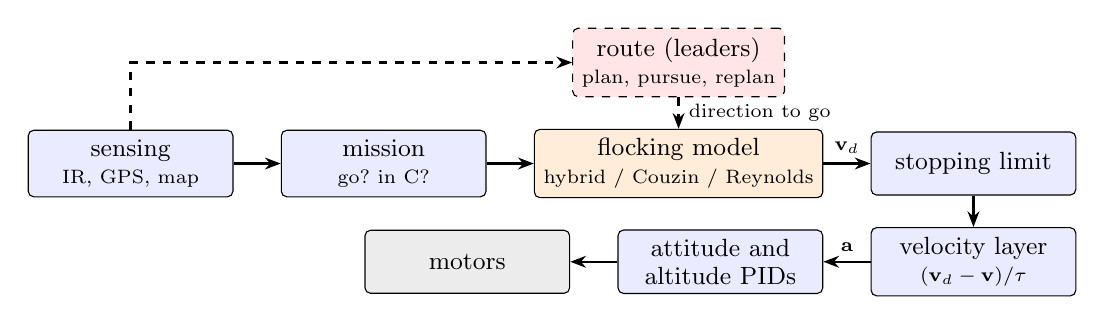
\begin{tikzpicture}[
    node distance=4mm and 6mm,
    layer/.style={draw, rounded corners=2pt, minimum height=8mm, minimum width=26mm,
                  align=center, font=\small, fill=#1},
    layer/.default=white,
    input/.style={align=center, font=\footnotesize},
    flow/.style={-{Stealth[length=2mm]}, thick},
  ]
  \node[layer=blue!8] (sense) {sensing\\[-1pt]\scriptsize IR, GPS, map};
  \node[layer=blue!8, right=of sense] (mission) {mission\\[-1pt]\scriptsize go?\ in C?};
  \node[layer=orange!15, right=of mission] (model) {flocking model\\[-1pt]
                                                   \scriptsize hybrid / Couzin / Reynolds};
  \node[layer=blue!8, right=of model] (limit) {stopping limit};
  \node[layer=blue!8, below=of limit] (velocity) {velocity layer\\[-1pt]
                                                  \scriptsize $(\mathbf v_d-\mathbf v)/\tau$};
  \node[layer=blue!8, left=of velocity] (attitude) {attitude and\\[-1pt]altitude PIDs};
  \node[layer=gray!15, left=of attitude] (motors) {motors};
  \node[layer=red!10, dashed, above=of model] (route) {route (leaders)\\[-1pt]
                                                      \scriptsize plan, pursue, replan};

  \draw[flow] (sense) -- (mission);
  \draw[flow] (mission) -- (model);
  \draw[flow] (model) -- node[above, font=\scriptsize] {$\mathbf v_d$} (limit);
  \draw[flow] (limit) -- (velocity);
  \draw[flow] (velocity) -- node[above, font=\scriptsize] {$\mathbf a$} (attitude);
  \draw[flow] (attitude) -- (motors);
  \draw[flow, dashed] (route) -- node[right, font=\scriptsize] {direction to go} (model);
  \draw[flow, dashed] (sense.north) |- (route.west);
\end{tikzpicture}

  \caption{One control step. Every drone hears its neighbours over infra-red
    and knows its own position and the walls; the flocking model turns that
    into a wanted velocity, which the lower layers fly. Only leaders have the
    route (dashed), which gives the model a direction to C.}
  \label{fig:layers}
\end{figure}

\paragraph{Sensing.} Each drone broadcasts its own velocity, in the world
frame, over an infra-red emitter every step. From each packet it receives, a
drone gets the sender's velocity, its distance (from the signal strength) and
its direction, which is rotated from the tilted body frame into the world
frame. Against the referee's ground truth, distances were off by 1.4\,cm on
average and directions by 0.4\textdegree. The IR carries 3\,m; a drone
considers neighbours within 2.5\,m. Its own position and velocity come from
GPS, and the walls from the map, given to every drone in the world file.
Neighbours are known only from IR and obstacles only from the map, so no
sensor has to correct another.

\paragraph{Mission.} A shared clock starts the trip: the flock forms for the
first 16\,s, all drones hovering by about 6\,s, and then the leaders set
off. A follower does not know where C is, but recognises it when it is inside
(on a real drone, a ground marker; here, GPS against C's rectangle). A drone
in C keeps cruising for 2.5\,m, so the flock fills C instead of piling up at
its edge, and then stops.

\paragraph{Route (leaders only).} At go time a leader plans a path to C on the
map and from then on follows it, planning again if the flock pushes it behind
a wall (\cref{sec:planner}). The route's only output is a direction and a
distance to go, which the model reads exactly as it would read the straight
line to C: with the planning layer off, a leader simply aims at C.

\paragraph{Flocking model.} From what the drone hears, its own velocity, the
mission state and, for a leader, the direction to go, the model computes a
\emph{wanted velocity}. Three models are interchangeable behind one interface
(\cref{sec:models}); everything around them is shared, so the experiments
compare the models and nothing else.

\paragraph{Stopping limit.} Shared by all models, it cuts the wanted velocity
down to what the drone could still brake from before reaching a wall, or a
neighbour, closer than 0.3\,m. It only removes speed, so it cannot push a
drone anywhere; it bounds whatever the model asks for.

\paragraph{Velocity and attitude.} The velocity layer turns the wanted
velocity $\mathbf{v}_d$ into an acceleration
$\mathbf{a} = (\mathbf{v}_d - \mathbf{v})/\tau$, capped at 2.5\,m/s$^2$, with
$\tau = 0.3$\,s, the fastest response measured to have no overshoot. The
acceleration becomes a tilt, which nested angle and rate loops hold as the
Crazyflie firmware does, under an altitude controller and the motor mixing.
\citet{viragh2014} describe a flying robot by exactly these imperfections, a
relaxation time and a maximum acceleration, and \cref{sec:controllers} shows
why they matter: rules that are stable for an ideal boid oscillated on the
drone until the robot could follow them.

\subsection{Choices and why}
\label{sec:choices}

\Cref{tab:choices} lists the choices that shape what the experiments can say,
each with the alternative turned down.

\begin{table}[tbp]
  \centering
  \small
  \begin{tabular}{@{}>{\raggedright\arraybackslash}p{0.27\linewidth}
                     >{\raggedright\arraybackslash}p{0.4\linewidth}
                     >{\raggedright\arraybackslash}p{0.27\linewidth}@{}}
    \toprule
    Choice & Why & Turned down \\
    \midrule
    Followers can't tell leaders from the others &
      Couzin's informed individuals \citep{couzin2005}: the research question
      is what unrecognised leaders can do &
      A leader flag in the IR packet \\
    \addlinespace
    Followers recognise C only when in it &
      Goal recognition, not goal knowledge: they stay uninformed, but a
      flock can stop at C &
      Followers that know C (no leaders needed) \\
    \addlinespace
    Alignment from broadcast velocities &
      A quadrotor flies sideways: its heading says nothing about its motion &
      Alignment with headings \\
    \addlinespace
    Obstacles from the map, position from GPS &
      The Crazyflie's four range rays leave blind spots and see flockmates as
      obstacles; \citet{vasarhelyi2018} also flew among virtual walls &
      On-board range sensing; mapping in flight (a project of its own) \\
    \addlinespace
    Models output a velocity, flown through $\tau$ and $a_{\max}$ &
      The robot is described by two measurable numbers, and every model meets
      the same robot &
      Accelerations straight to tilt \\
    \addlinespace
    Each leader plans on board, for itself &
      A leader that deliberates, from where it is, with what it knows &
      Paths computed by the world generator and handed out \\
    \addlinespace
    Separate seeds for the map and the run &
      Results can't change because the course did &
      One seed for both \\
    \bottomrule
  \end{tabular}
  \caption{Design choices, from the design log.}
  \label{tab:choices}
\end{table}

\subsection{Tools}
\label{sec:tools}

Around the controllers, a small set of tools runs the experiments, all in the
same repository:
\begin{itemize}
  \item \texttt{make\_world.py} builds a world from a map, $n$, $j$ and a
        seed, to open in Webots and watch;
  \item a headless runner starts Webots without a window, runs a world until
        a condition holds, and stops it; an 83\,s run of 10 to 30 drones
        took under a minute of wall-clock time (median 49\,s);
  \item \texttt{sweep.py} runs every combination of $n$, $j$ and seed for a
        model and appends one row per run (time to 90\% in C, drones in C at
        the end, the closest two drones came, crashes, \ldots) to a CSV file;
        a stopped sweep resumes where it left off;
  \item \texttt{tune.py} runs a grid of model settings on seeds kept apart
        from the experiments;
  \item \texttt{analyse.py} computes every number and figure in
        \cref{sec:results} from those files.
\end{itemize}
Any setting of any layer can be changed for one run from the command line,
so an experiment never needs an edited source file. The code (about 3000
lines) is covered by 212 unit tests, checked by a linter and a type checker
on every push.

\section{Controllers}
\label{sec:controllers}

This section describes the three parts of the controller the project
designed: the flight layer that lets a drone follow a flocking model, the three
models, and the leaders' planning layer. Each part reached its form through
failures observed in simulation; the main ones are told here, because they
explain the design.

\subsection{Flight: the ideal boid is not the robot}
\label{sec:flight}

The first version turned each boid acceleration straight into a tilt and
flew Reynolds' rules unchanged. Twenty drones hovered calmly, then
neighbouring pairs started swinging in and out with a period of about 2\,s,
wider each time, until two touched and the physics blew up. The rules assume
a boid accelerates the moment it is asked to; a quadrotor has to tilt first,
and the attitude controller, with the gains of the Webots example, was slow
and underdamped (a tilt step overshot by 45\%). A stiff spring, separation
growing as $1/d^2$, behind a lagging, resonant actuator oscillates.
\citet{viragh2014} report the same delay-induced oscillations in flying
robots, colliding even in a hovering flock, and describe a robot by exactly
such imperfections.

So the drone was made to follow first, before touching the rules:
\begin{itemize}
  \item attitude is held by two nested loops, as in the Crazyflie firmware:
        the angle error sets a wanted rotation rate, capped at 1.5\,rad/s,
        and the rate error sets the motor differential. Faster rotations
        flipped the drone in hard reversals. A 21\textdegree\ tilt step now
        reaches 90\% in 0.26\,s with 4\% overshoot, where before it never
        did within a second;
  \item the hover speed comes from the physics ($4k\omega^2 = mg$, so
        $\omega = 55.4$\,rad/s, against 55.37 measured), and the motors speed
        up by $1/\sqrt{\cos\phi\cos\theta}$ when tilted;
  \item every model outputs a wanted velocity $\mathbf v_d$, which a velocity
        layer flies as $\mathbf a = (\mathbf v_d - \mathbf v)/\tau$, capped at
        $a_{\max} = 2.5$\,m/s$^2$. Velocity steps measured against a point
        mass with the same $\tau$ showed that below $\tau \approx 0.3$\,s the
        response stops getting faster, since that is the attitude loops' own
        speed, and only overshoots; $\tau = 0.3$\,s is the fastest setting
        without overshoot.
\end{itemize}
The attitude loops alone were enough for the same rules, unchanged, to settle
into a calm lattice with no collision (closest pair 0.64\,m, against contact
before). The velocity layer came later, with the hybrid model, whose terms are
velocities; it describes the robot by two measured numbers, $\tau$ and
$a_{\max}$, so every model meets the same robot.

\subsection{Three flocking models}
\label{sec:models}

\paragraph{Notation.} For drone $i$, $\mathcal N_i$ are the neighbours it
hears within the perception radius $\rho = 2.5$\,m; $\mathbf d_{ij}$ is the
offset from $i$ to $j$, $d_{ij} = |\mathbf d_{ij}|$, and $\hat{\mathbf x}$ is
the unit vector of $\mathbf x$. $\mathbf v_i$ is a drone's velocity and
$\mathbf g_i$, for a leader, the direction to go, from the route
(\cref{sec:planner}) or straight at C, with $|\mathbf g_i|$ the distance left.
$v_0 = 1$\,m/s is the cruise speed. Every speed in the models is a multiple of
$v_0$ (rates scale with it, decelerations with its square), so the rules are
exactly speed-free: at $k$ times $v_0$ the same flock flies the same paths, $k$
times as fast. A test checks this.

All three models share everything but the social rule: the mission clock, the
stopping limit, the flight layer, perception, $v_0$, and which drones lead.
Their leaders all slow down within $r_{\mathrm{arr}} = 3$\,m of C, by
$s_i = \min(1, |\mathbf g_i|/r_{\mathrm{arr}})$, so they stop there.

\paragraph{Reynolds.} The rules of \citet{reynolds1987} give an acceleration:
\begin{equation}
  \mathbf a_i =
    k_s \!\!\sum_{j:\,d_{ij} < r_s}\!\! \Bigl(\frac{r_s}{d_{ij}} - 1\Bigr)(-\hat{\mathbf d}_{ij})
  + k_a \bigl(\overline{\mathbf v}_j - \mathbf v_i\bigr)
  + k_c\, \overline{\mathbf d}_{ij}
  \;\bigl[\, + k_g\,(v_0 s_i \hat{\mathbf g}_i - \mathbf v_i) \text{ for a leader}\bigr],
\end{equation}
separation, alignment with the neighbours' mean velocity, cohesion toward
their centre, and, for leaders, Reynolds' seek and arrive. The wanted
velocity $\mathbf v_d = \mathbf v_i + \tau \mathbf a_i$ makes the velocity
layer fly exactly $\mathbf a_i$. Nothing propels a follower: it moves only as
its neighbours pull it. Parameters: $r_s = 1$\,m, $k_s = 4$\,m/s$^2$,
$k_a = 4$\,s$^{-1}$, $k_c = 1.2$\,s$^{-2}$, $k_g = 4$\,s$^{-1}$.

\paragraph{Couzin.} In the zone model of \citet{couzin2002}, as used by
\citet{couzin2005}, each drone keeps a direction $\hat{\mathbf u}_i$ as its
own state and flies it at $v_0$. If any neighbour is inside the zone of
repulsion $\alpha$, avoiding them is all that counts; otherwise attraction and
alignment weigh each neighbour the same:
\begin{equation}
  \mathbf u_i \leftarrow
  \begin{cases}
    -\sum_{j:\,d_{ij} < \alpha} \hat{\mathbf d}_{ij} & \text{if any } d_{ij} < \alpha,\\[2pt]
    \sum_{j} \hat{\mathbf d}_{ij} + \sum_{j \text{ moving}} \hat{\mathbf v}_j
      + \hat{\mathbf u}_i & \text{otherwise.}
  \end{cases}
\end{equation}
An informed individual adds the goal with weight $\omega$,
$\hat{\mathbf u}_i \leftarrow \mathrm{unit}(\hat{\mathbf u}_i + \omega \hat{\mathbf g}_i)$,
and the wanted velocity is $v_0 s_i \hat{\mathbf u}_i$. Parameters:
$\alpha = 0.4$\,m, $\omega = 1$; the zones of orientation and attraction
merge into the perception radius. Two departures from the papers, both
deliberate: a follower has no direction until a neighbour moves (Couzin's
agents start with random ones, which would scatter the swarm at the start),
and the turning-rate limit and noise are left to the real drone.

\paragraph{Hybrid.} The model of \citet{vasarhelyi2018}, designed for real
drones, with Reynolds' cohesion and Couzin's informed leaders. Its terms are
velocities:
\begin{equation}
  \mathbf v_d = v_0 \hat{\mathbf h}_i
  + p_r \!\!\sum_{j:\,d_{ij} < r_0}\!\! (r_0 - d_{ij})(-\hat{\mathbf d}_{ij})
  + C_f \sum_j \bigl(|\mathbf v_{ij}| - D_{ij}\bigr)^{+}\, \hat{\mathbf v}_{ij}
  + p_c\, \overline{\mathbf d}_{ij},
\end{equation}
cruise, linear repulsion, friction and cohesion, with
$\mathbf v_{ij} = \mathbf v_j - \mathbf v_i$. Friction is Vásárhelyi's
velocity alignment: two neighbours may differ in velocity by
$D_{ij} = \max\bigl(v_s, D(d_{ij} - r_f)\bigr)$, and only the excess is
corrected. The braking curve
\begin{equation}
  D(x) =
  \begin{cases}
    0 & x \le 0,\\
    p\,x & 0 < p\,x < a/p,\\
    \sqrt{2ax - a^2/p^2} & \text{otherwise}
  \end{cases}
\end{equation}
is the highest speed from which a drone can still stop within $x$, at
deceleration $a$, gentler over the last stretch. Alignment is thus strong up
close and slack far away. The cruise heading $\hat{\mathbf h}_i$ is the mean
direction of the neighbours seen moving, the drone's own included, Couzin's
zone of orientation; a leader uses the same mean without itself, mixed with
the goal, $\mathrm{unit}(\hat{\mathbf h}_i + w\hat{\mathbf g}_i)$, and cruises at
$v_0 s_i$. Parameters, scaled from the authors' simulator to our speed and
spacing and then tuned: $r_0 = 1$\,m, $p_r = 1$\,s$^{-1}$, $C_f = 0.2$,
$v_s = 0.12\,v_0$, $r_f = 2$\,m, $p = 1$\,s$^{-1}$, $a = 1.6$\,m/s$^2$,
$p_c = 0.4$\,s$^{-1}$, $w = 1$.

\paragraph{How the hybrid got its shape.} The hybrid is the model the project
grew on \texttt{l\_hall}, and each of its departures from Vásárhelyi's model
answers a failure seen there:
\begin{itemize}
  \item \emph{Friction gain 0.2, not 1.} Friction sums over about ten
        neighbours, so at gain 1 a drone tries to correct a velocity
        difference ten times faster than it can tilt; a resting flock
        jiggled at 0.2\,m/s. At 0.2 it settles.
  \item \emph{A stopping limit instead of walls that push.} Vásárhelyi keeps
        drones off walls with virtual agents that push them away. A pillar
        forest then looked like a solid wall, and the push, faster than the
        cruise, bounced the flock back. The stopping limit below replaced it.
  \item \emph{The heading is alignment.} At first each drone cruised along
        its own last heading. Eighteen private headings outvoted two leaders:
        drones that slid into a corner stayed there, and one leader flew away
        from C. Couzin's result relies on followers having no direction of
        their own beyond their neighbours', and his informed individual mixes
        the goal with the social direction, not with its own momentum. With
        the heading taken from the neighbours, the flock wakes from its
        leaders outward.
\end{itemize}

\paragraph{The stopping limit.} Every model's wanted velocity ends in the same
limit: toward each neighbour, beyond that neighbour's own speed away, and
toward each wall, a drone may close only as fast as it could still stop
before a margin $m = 0.3$\,m:
\begin{equation}
  \mathbf v_d \cdot \hat{\mathbf d}_{ij} \le
    \mathbf v_j \cdot \hat{\mathbf d}_{ij} + D(d_{ij} - m),
  \qquad
  \mathbf v_d \cdot \hat{\mathbf w} \le D(d_w - m).
\end{equation}
Each inequality is a half-plane of allowed velocities; a few rounds of
projecting onto them in turn find a velocity inside all of them. The walls
get the last rounds, so where the limits conflict the wall's is the one kept:
a drone caught between a wall and a closing neighbour may end up too close to
the neighbour, but never in the wall. The limit only removes
speed, so nothing bounces, and it bounds whatever a model asks for. On the
real dynamics it kept drones about 0.3\,m from walls; between drones, in a
crowd, it did not always hold (\cref{sec:results}).

\paragraph{Tuning.} The hybrid was tuned over the whole of its development on
\texttt{l\_hall}. To compare it fairly, Couzin and Reynolds were then tuned
on the same map under one protocol, fixed before any run: two settings each,
chosen from how the model had failed, 15 runs each (a grid on one seed, the
best three again on a second), on seeds never used by the experiments, scored
by the drones in C at the end. Couzin's best was $\omega = 1$,
$\alpha = 0.4$\,m: a wider zone of repulsion, which overrides everything
else, held the drones apart too long at the gap. Reynolds' best, goal 4 and
alignment 4, brought 1 drone of 20 to C: its leaders stop at the L's inner
corner, where steering straight at C presses them into a wall, a local
minimum no weight removes. A later check with the plan on as well left
$\omega$ at 1, but showed that a Couzin leader off the walls can leave its
flock behind for good, since nothing holds it to the flock's pace. That is a
property of the model as published, kept and measured
(\cref{sec:results}).

\subsection{The leaders' planning layer}
\label{sec:planner}

A leader that steers straight at C fails wherever that line crosses a wall:
Reynolds' leaders stopped at the L's inner corner, and on \texttt{dead\_end}
every model's flock ends in the cup. The leaders therefore get a deliberative
layer on top of the reactive model, the hybrid architecture of
\citet{arkin1998}: a leader plans a path on the known map and follows it,
while the flocking model stays as it is. Followers are untouched: they don't
know a map exists, so the leadership question stays the same, and only what a
leader knows changes.

\paragraph{What a leader plans around.} The arena's outline and every obstacle
at least 1\,m across. Smaller obstacles, such as \texttt{l\_hall}'s pillars,
are left to the stopping limit, since a flock flows through a forest that a
planner would have to treat as a wall.

\paragraph{Path finding.} No single clearance works: a large one erases the
passages drones fly through, a small one makes the path hug every corner and
drag the flock into it. So the clearance is a cost, not a constraint: A*
\citep{hart1968} on a grid of 0.25\,m cells, 8-connected, where cells closer
than the drones' margin (0.3\,m) to an obstacle are forbidden and a step at
distance $d < c = 2$\,m from the nearest one costs
\begin{equation}
  1 + w \left(\frac{c - d}{c - m}\right)^{2}, \qquad w = 4,
\end{equation}
times its length. In a hall 8\,m wide the centre line is free, a 4\,m gap is
crossed through its middle, and a narrower passage is still allowed, at a
price (\cref{fig:maps}). The path is then pruned to its corners: a shortcut
between two waypoints is kept only if it never comes closer to a wall than the
planned path between them did, so pruning cannot undo the clearance. Turned
down: a visibility graph (it needs the one clearance we can't choose),
Voronoi roadmaps (maximal clearance, long detours in open rooms) and sampling
planners such as RRT (built for many dimensions, and random).

\paragraph{Path following.} The leader aims at the point 2\,m ahead along its
path from wherever the flock has pushed it, pure pursuit \citep{coulter1992};
its progress along the path only moves forward, so a path that doubles back
is not cut short. The route hands the model $\mathbf g_i$: the direction to
that point, with the length of the path still to go, so the models' own
arrive term still stops the leader at C and no model had to change.

\paragraph{Planning again.} A leader first planned once, at go time, from
where it hovered. Replays of the failures on \texttt{dead\_end} showed why
that was not enough: the flock had pushed a leader into the cup, its lookahead
point lay on the other side of the cup's arm, and pursuing it pressed the
leader into the wall. Now, whenever the lookahead point is hidden behind a
kept obstacle, the leader plans again from where it is, at most once a
second. The line-of-sight test is exact: a segment clipped against each box
\citep{liang1984} and its distance to each pillar's centre. On every run that
succeeded with a single plan, replanning never triggered: those runs ended at
the same time to the millisecond. It changed only the failures.

\paragraph{Each leader for itself.} Every leader plans its own path from its
own position, with no exchange with the others: a leader that deliberates
with what it knows. Where an obstacle can be passed on either side, two
leaders may choose different sides. This was expected to split the flock at
worst, with each part keeping a leader; \cref{sec:results} shows that for one
model it does something else.

\todo{Video: dead\_end with the plan off (the flock fills the cup) and on,
with a replan.}

\section{Experimental method}
\label{sec:method}

% Slides 1.3 and 2.9: define objectives and hypotheses, the setting, the
% measure, then analyse with statistics and plots.

\subsection{Setting}
% Maps: tuned on l_hall, evaluated on dead_end and l_turn, which no model
% was tuned on (avoids the tuning-map confound). Seeds 0-9: each seed is
% one spawn, shared by every model and setting, so runs pair by seed.
% Two experiments: (1) the evaluation, n = 20, j = 2, model x plan on both
% held-out maps; (2) the sweep, dead_end with the plan, n x j x model.
\todo{Maps, seeds, the two experiments.}

\subsection{Measure}
% Success: 90% of the drones in C within the limit, go time + twice the
% leaders' own time along their planned path (83 s on dead_end, 112 s on
% l_turn). Why a limit: a flock that lost its leaders wanders into C by
% chance given time (false positives, design log 2026-10-28). Why twice:
% larger flocks pass gaps slower. Also logged: time to 90%, the closest
% two drones came, crashes.
\todo{Success within the limit; secondary measures.}

\subsection{Statistics}
% Paired by seed. Success is binary: exact McNemar test (binomial on the
% discordant seeds). Closest pair: Wilcoxon signed-rank. Leader split:
% Fisher's exact test. Uncorrected p, many comparisons: read as evidence,
% not proof. With 10 seeds the smallest McNemar p is 0.002.
\todo{Tests and their limits.}

\subsection{Traps, and how they were handled}
% Nehmzow's traps (slides 1.3):
%   confounds -> held-out maps; models tuned by the same protocol;
%   floor/ceiling -> l_turn is at the ceiling, dead_end separates; the
%     j = 0 control fixes the floor;
%   systematic errors -> identical spawns per seed across models;
%   wishful thinking -> hypotheses before the sweep, the limit kept when
%     it cost results ("Too hard a limit? Checked, kept").
\todo{Traps.}

\section{Results}
\label{sec:results}

Every number in this section is computed by \texttt{tools/analyse.py} from the
runs' logs; the design log (28 and 29 October) records how each was first
read.

\subsection{Evaluation: model and plan}
\label{sec:evaluation}

\Cref{tab:evaluation} gives the evaluation: 20 drones and 2 leaders on the
two held-out maps.

\begin{table}[tbp]
  \centering
  \small
  \begin{tabular}{@{}lcccc@{}}
    \toprule
    & \multicolumn{2}{c}{\texttt{dead\_end} (83\,s)} & \multicolumn{2}{c}{\texttt{l\_turn} (112\,s)} \\
    \cmidrule(lr){2-3}\cmidrule(l){4-5}
    & plan off & plan on & plan off & plan on \\
    \midrule
    hybrid   & 0/10        & 2/10 (47\,s) & 10/10 (68\,s) & 10/10 (66\,s) \\
    Couzin   & 3/10 (73\,s) & 6/10 (57\,s) & 9/10 (75\,s)  & 9/10 (75\,s) \\
    Reynolds & 0/10        & 8/10 (56\,s) & 0/10          & 10/10 (69\,s) \\
    \bottomrule
  \end{tabular}
  \caption{Evaluation, 20 drones, 2 leaders: runs out of 10 seeds with 90\% of
    the drones in C within the limit, and the median time to 90\% of those
    runs.}
  \label{tab:evaluation}
\end{table}

\paragraph{The plan.} With the plan, Reynolds' flock reaches C in 8 of 10 runs
on \texttt{dead\_end} and in all 10 on \texttt{l\_turn}, from none on either
map without it (paired: 8 seeds to none, $p = 0.008$; 10 to none,
$p = 0.002$). This confirms H2: the trap at the corner is steering straight at
C, not Reynolds' rules, since the same rules get round it as soon as the
leaders follow a path. For the hybrid and Couzin the plan's effect is small
(2 seeds to none, and 4 to 1, $p \ge 0.37$): on \texttt{l\_turn} both already
succeed without it, because their flocks' own momentum carries the leaders
round the corner; on \texttt{dead\_end} the hybrid stays low either way. H1
holds for Reynolds and is not shown for the other two; its second part, no
effect where the way to C is clear, was not tested.

\paragraph{The models.} With the plan off, the hybrid and Couzin beat Reynolds
on \texttt{l\_turn} (10 and 9 seeds to none, $p \le 0.004$). With the plan on,
the order on \texttt{dead\_end} reverses: Reynolds 8, Couzin 6, the hybrid 2.
Hybrid against Reynolds is 6 seeds to none ($p = 0.03$). In the hybrid's 8
failures only 1 or 2 drones, its leaders, are in C at the limit:
\cref{sec:split} shows why. Couzin succeeds where the other two don't with
the plan off (3 runs), and loses its flock in a few runs with the plan on, as
expected from its tuning: its leaders, off the walls, can leave the flock
behind.

\paragraph{Spacing.} \Cref{fig:evaluation-closest} shows the closest two
drones came in each run. Reynolds keeps its drones apart, 0.42--0.51\,m in
median, never closer than 0.33\,m. The hybrid and Couzin crowd to touching
distance, 0.10\,m, in many runs, and Couzin is the only model that crashed (4
runs of 40; the plan-off runs were measured over 200\,s). So H3 holds for
reaching C, where tuned Couzin matches the hybrid, but not for spacing:
Couzin's drones are no further apart than the hybrid's. The plan widens the
hybrid's spacing on both maps (Wilcoxon, $p \le 0.004$): a flock that presses
into a wall is a compressed flock.

\begin{figure}[tbp]
  \centering
  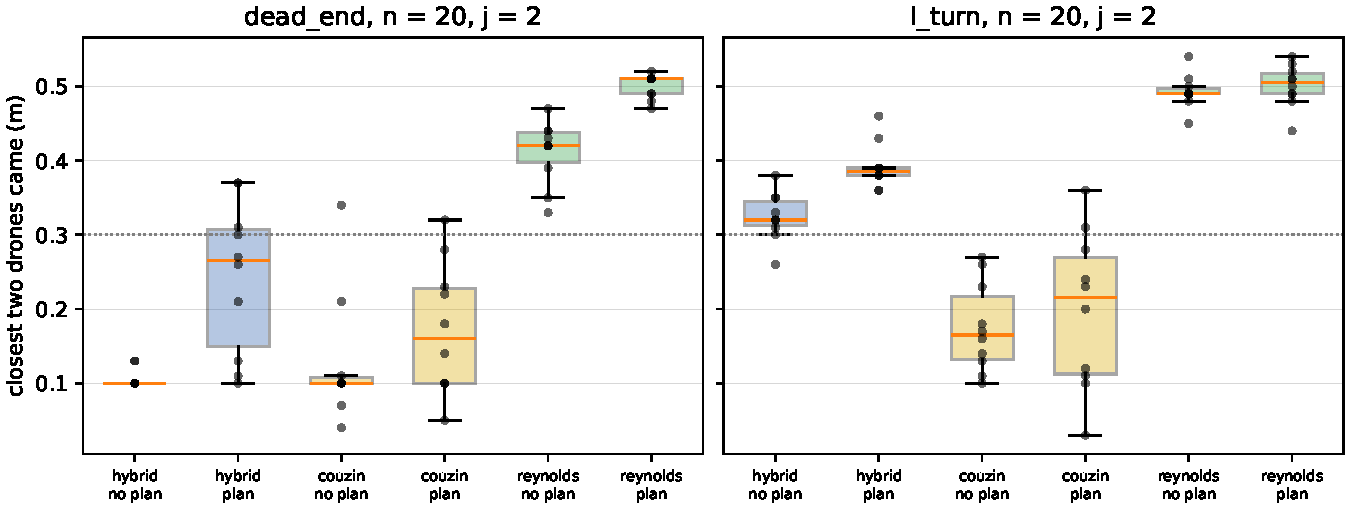
\includegraphics[width=\linewidth]{evaluation_closest}
  \caption{The closest two drones came in each run, on the held-out maps with
    20 drones and 2 leaders, 10 seeds. Dotted: the 0.3\,m stopping margin;
    0.10\,m is touching.}
  \label{fig:evaluation-closest}
\end{figure}

\subsection{Drones and leaders}
\label{sec:sweep}

\Cref{fig:sweep-success} shows the second experiment, on \texttt{dead\_end}
with the plan on, and \cref{tab:leaders} pools it over the three flock sizes.

\begin{figure}[tbp]
  \centering
  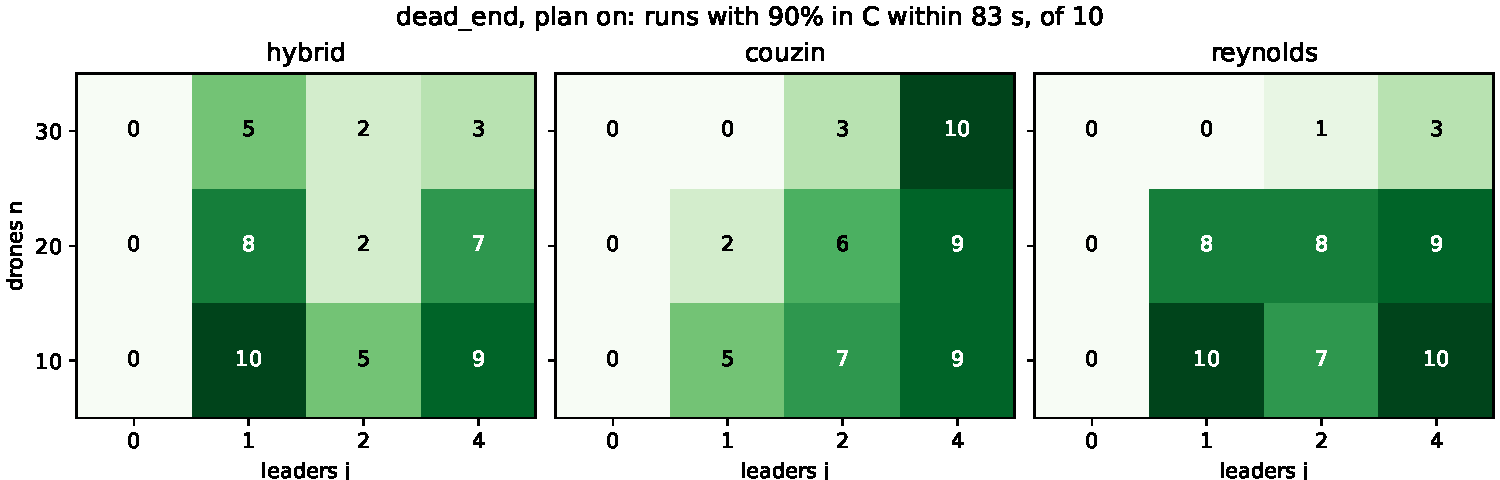
\includegraphics[width=\linewidth]{sweep_success}
  \caption{\texttt{dead\_end} with the plan: runs out of 10 seeds with 90\% of
    the drones in C within 83\,s, by flock size $n$ and leaders $j$.}
  \label{fig:sweep-success}
\end{figure}

\begin{table}[tbp]
  \centering
  \small
  \begin{tabular}{@{}lccccl@{}}
    \toprule
    & $j = 0$ & $j = 1$ & $j = 2$ & $j = 4$ & paired, $j = 1$ vs 4 \\
    \midrule
    hybrid   & 0/30 & 23/30 & 9/30  & 19/30 & 4 / 8 seeds, $p = 0.39$ \\
    Couzin   & 0/30 & 7/30  & 16/30 & 28/30 & 22 / 1 seeds, $p < 10^{-5}$ \\
    Reynolds & 0/30 & 18/30 & 16/30 & 22/30 & 5 / 1 seeds, $p = 0.22$ \\
    \bottomrule
  \end{tabular}
  \caption{\texttt{dead\_end} with the plan, pooled over $n = 10, 20, 30$:
    successful runs out of 30, and the paired test of 1 leader against 4
    (seeds won by $j = 4$ / by $j = 1$).}
  \label{tab:leaders}
\end{table}

\paragraph{No leaders, no arrival.} None of the 90 runs with $j = 0$ reached C
within the limit. Every success in the experiment is the leaders' doing: the
chance level the time limit was set to remove is zero.

\paragraph{More leaders.} Couzin's model behaves as \citet{couzin2005}
predict: its flock follows more reliably the more leaders it has, 7, 16 and
28 runs of 30 for 1, 2 and 4 leaders (from 1 to 2: 11 seeds to 2,
$p = 0.02$; from 2 to 4: 13 to 1, $p = 0.002$), and at $n = 30$ it is the
only model that still succeeds reliably, 10 of 10 with 4 leaders against 3 for
the other two. With one leader its flock packs to touching distance and does
not follow. Reynolds hardly depends on $j$ (18, 16, 22 of 30; every pair
$p \ge 0.07$). The hybrid does worse with 2 leaders than with 1: 23 of 30
against 9, 14 seeds to none ($p = 0.0001$), and recovers with 4. H4 holds for
Couzin's model only.

\paragraph{Larger flocks.} Every model succeeds less with more drones (over
$j > 0$: the hybrid 24, 17, 10 runs of 30 from $n = 10$ to 30; Couzin 21, 17,
13; Reynolds 27, 25, 4). With $j$ fixed, the fraction of leaders falls as $n$
grows, so this does not contradict Couzin's result that larger groups need a
\emph{smaller fraction}; it says that, here, they need more than a constant
number. Reynolds' collapse at $n = 30$ is the sharpest: from 25 of 30 to 4.

\paragraph{Cost.} \Cref{fig:sweep-cost} shows what success costs. Reynolds
arrives in about the same time as the others (median 51--54\,s against
47--60\,s) with its drones twice as far apart (median closest pair about
0.5\,m). Couzin with one leader sits at 0.10\,m; with more leaders its
spacing widens to the hybrid's. The hybrid with 4 leaders is the slowest
(median 60\,s).

\begin{figure}[tbp]
  \centering
  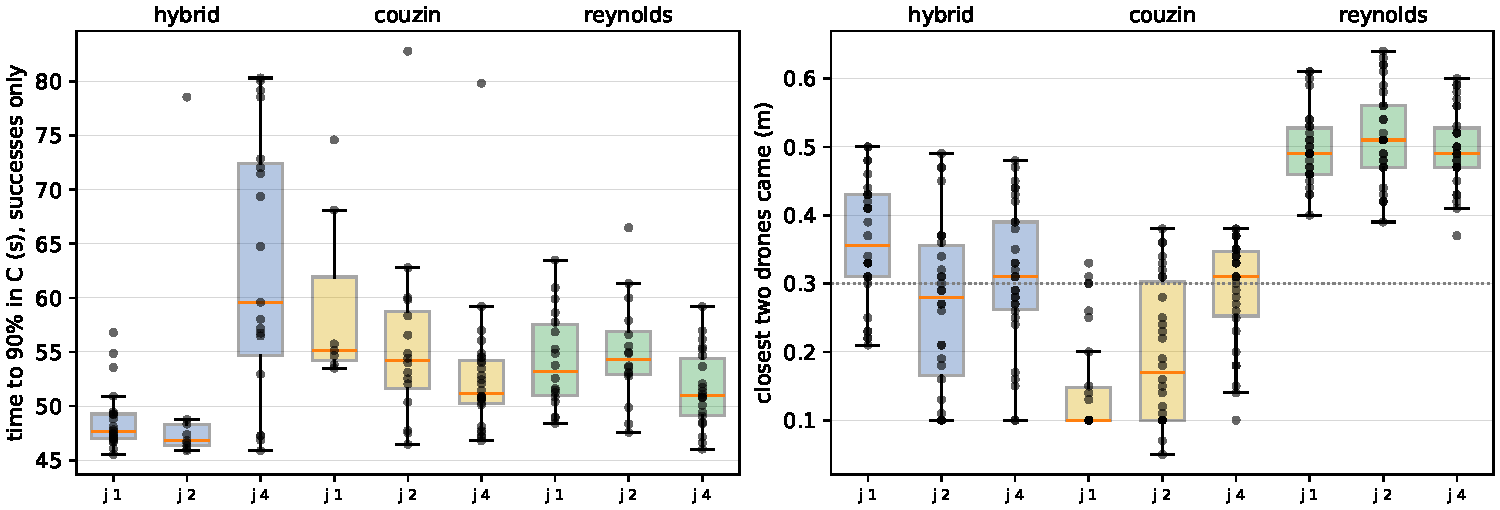
\includegraphics[width=\linewidth]{sweep_cost}
  \caption{\texttt{dead\_end} with the plan, pooled over flock sizes: the time
    to 90\% in C of the successful runs (left) and the closest two drones came
    in every run (right), per model and number of leaders.}
  \label{fig:sweep-cost}
\end{figure}

\subsection{Why two leaders lose the hybrid's flock}
\label{sec:split}

A failure of the hybrid with 2 leaders that Reynolds, on the same spawn,
turns into a success, replayed and drawn in \cref{fig:split}, shows the
mechanism.

\begin{enumerate}
  \item The two leaders start on either side of the cup's axis, and each
        plans round its own arm of the cup, one over the top, one under the
        bottom. Their paths part slowly, so at go time both still head
        roughly east.
  \item The hybrid's followers cruise along the mean heading of their
        neighbours, and they are at full speed within 2\,s of the start. The
        two leaders' pulls, up and down, cancel, so the followers fly straight
        on, overtake both leaders and fill the cup.
  \item At the bottom of the cup they turn back as one, carry the top leader
        with them (a leader mixes the goal with its neighbours' heading), and
        loop round the room. The bottom leader reaches C alone.
  \item Reynolds' followers have no cruise: they speed up only as their
        neighbours pull them (0.34\,m/s at 18\,s, against the hybrid's
        0.99). The leaders get ahead and apart before the flock commits, and
        the flock goes with one of them, over the top arm, into C.
\end{enumerate}

This is the averaging \citet{couzin2005} found in groups with two informed
subgroups: when their preferred directions differ only a little, the group
follows their mean, and only a wide enough difference makes it choose one.
Here the difference starts small, two paths that part slowly, and their mean
leads into the dead end.

\begin{figure}[tbp]
  \centering
  \begin{subfigure}{\linewidth}
    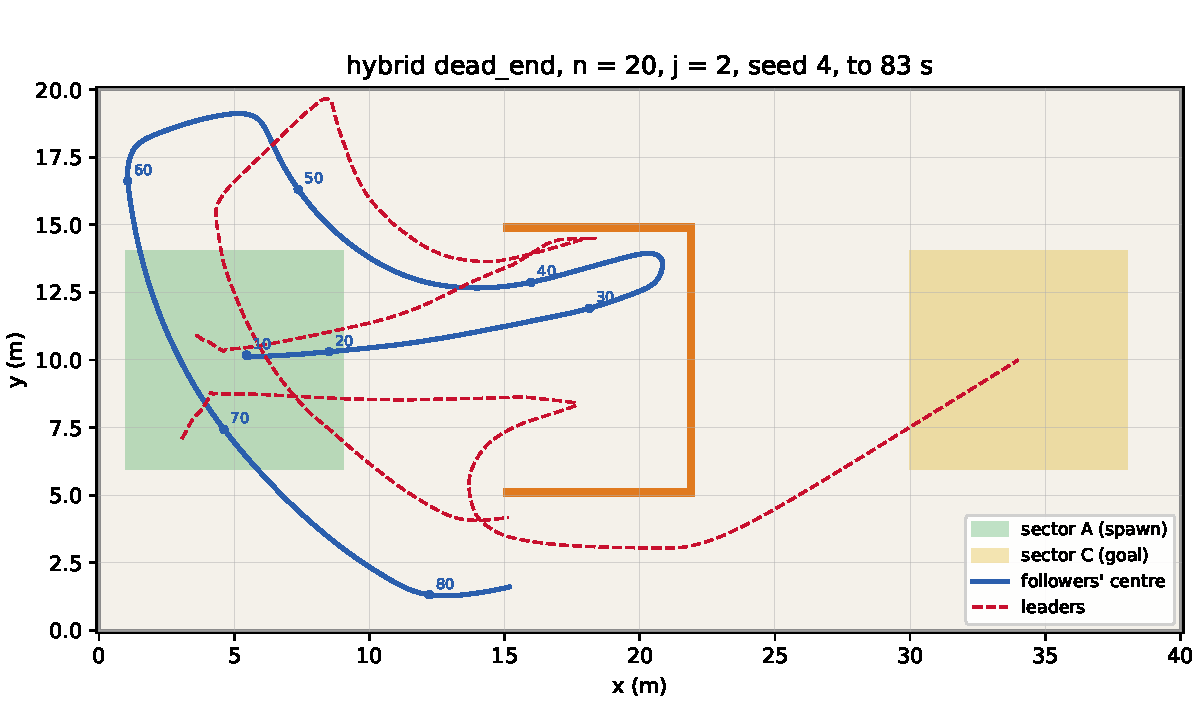
\includegraphics[width=\linewidth]{trajectory_dead_end_hybrid_plan_n20_j2_seed4}
    \caption{Hybrid: the followers fly between the two leaders into the cup,
      then loop round the room with the top leader.}
  \end{subfigure}
  \begin{subfigure}{\linewidth}
    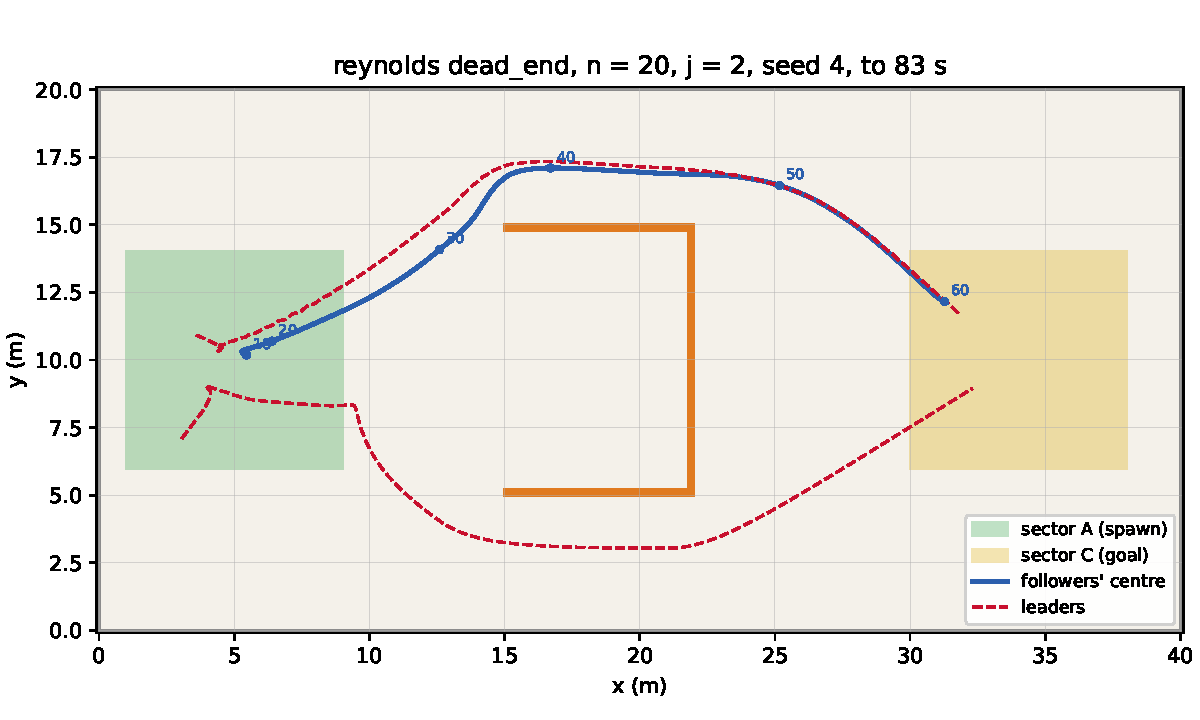
\includegraphics[width=\linewidth]{trajectory_dead_end_reynolds_plan_n20_j2_seed4}
    \caption{Reynolds: the followers go with the top leader into C.}
  \end{subfigure}
  \caption{The same spawn (seed 4, 20 drones, 2 leaders) with two models, to
    the 83\,s limit. Solid: the followers' centre, numbered every 10\,s;
    dashed: the leaders.}
  \label{fig:split}
\end{figure}

\paragraph{Over all runs.} A* is deterministic and a leader plans from within
a metre of where it spawned, so planning from each leader's spawn tells which
way it went. \Cref{tab:split} relates that to success for the runs with 2
leaders.

\begin{table}[tbp]
  \centering
  \small
  \begin{tabular}{@{}lccc@{}}
    \toprule
    & same way (10 runs) & opposite ways (20 runs) & Fisher's exact $p$ \\
    \midrule
    hybrid   & 7/10 & 2/20  & 0.002 \\
    Couzin   & 7/10 & 9/20  & 0.26 \\
    Reynolds & 5/10 & 11/20 & 1.0 \\
    \bottomrule
  \end{tabular}
  \caption{\texttt{dead\_end} with the plan, 2 leaders, $n = 10, 20, 30$:
    successful runs when both leaders plan round the same side of the cup and
    when they plan round opposite sides.}
  \label{tab:split}
\end{table}

Only the hybrid is broken by the split: with its leaders on one side it
succeeds as often as the others. Couzin's and Reynolds' flocks choose a
leader. With 4 leaders the hybrid recovers (19 of 30); an even 2--2 split
does not break it the same way (8 of 12 runs), which this analysis does not
explain.

\todo{Video: the hybrid and Reynolds on seed 4, side by side.}

\section{Discussion}
\label{sec:discussion}

\subsection{The hypotheses}
\label{sec:verdicts}

\begin{table}[tbp]
  \centering
  \small
  \begin{tabular}{@{}>{\raggedright\arraybackslash}p{0.2\linewidth}
                     >{\raggedright\arraybackslash}p{0.17\linewidth}
                     >{\raggedright\arraybackslash}p{0.55\linewidth}@{}}
    \toprule
    Hypothesis & Verdict & Evidence \\
    \midrule
    H1, planning & holds for Reynolds &
      Reynolds 0 $\to$ 8 and 0 $\to$ 10 of 10; hybrid and Couzin within 4
      seeds. The ``no effect where the way is clear'' half was not tested. \\
    \addlinespace
    H2, the corner trap & holds &
      Reynolds never got round with the plan off, in tuning or evaluation;
      with the plan, 10 of 10 on \texttt{l\_turn}. \\
    \addlinespace
    H3, tuned Couzin & half &
      Reaches C as often as the hybrid; its drones touch as the hybrid's do,
      and it is the only model that crashed. \\
    \addlinespace
    H4, leaders & Couzin only &
      Couzin 7, 16, 28 of 30 for 1, 2, 4 leaders; Reynolds flat; the hybrid
      worst with 2. \\
    \bottomrule
  \end{tabular}
  \caption{The hypotheses of \cref{sec:hypotheses} against the results.}
  \label{tab:verdicts}
\end{table}

\Cref{tab:verdicts} closes the loop. Two hypotheses hold, one half holds,
and the research question of the project, H4, holds for one model out of
three. The rest of this section argues that these are not three separate
outcomes but one.

\subsection{What drives a follower}
\label{sec:drive}

The three models differ in many terms, but one difference explains most of
the results: what makes a follower move.

\begin{description}
  \item[Hybrid: its own cruise.] A follower cruises at full speed along its
    neighbours' mean heading. The flock therefore has momentum. On
    \texttt{l\_turn} that momentum carries the leaders round the corner even
    with no plan, where Reynolds' leaders stop (10 of 10 against none). On
    \texttt{dead\_end} the same momentum is the problem: two leaders heading
    round opposite arms of the cup pull the mean heading two ways, the pulls
    cancel, and the flock cruises on between them, into the cup. The flock is
    quick to follow a heading, and so it follows the average one.
  \item[Reynolds: nothing but its neighbours.] A follower has no drive of its
    own; it moves only as its neighbours pull it. With leaders that steer
    straight at C, that is useless: the leaders stop at a wall and the flock
    stops with them. With leaders that follow a plan, it is faithful: the
    flock speeds up slowly, the leaders get ahead before it commits, and when
    two leaders disagree the flock goes with one of them. Reynolds' success
    hardly depends on the number of leaders, presumably because one leader
    pulling is enough for a flock that has nothing pulling it the other way.
  \item[Couzin: a direction to be outvoted.] A follower keeps a direction as
    its own state and turns it toward its neighbours'. Leaders have to outvote
    the flock, so more leaders work better, exactly as
    \citet{couzin2005} predicted; one leader among 30 is lost. And since a
    Couzin leader feels its flock only while it still sees it, a leader that
    gets ahead can leave the flock behind for good.
\end{description}

So no model is simply best. Each one's strength and its weakness come from the
same property. Momentum makes the hybrid robust to leaders that steer badly
and fragile to leaders that disagree; having no drive makes Reynolds' flock
useless without a plan and faithful with one; state makes Couzin's flock
need enough leaders and lets its leaders run away. Which model to choose
depends on what the leaders can be trusted to do.

\subsection{A plan helps only if the flock follows}
\label{sec:plan-and-flock}

The planning layer was designed for the leaders alone, and on that level it
works: in the replays, no leader stayed stuck in the cup once it could plan
again. But a better path for the leaders helps only as far as the flock
follows them, and the model decides that. The leaders also plan
independently, as if they were interchangeable: each from where it stands,
each for itself. This was expected to split the flock at worst, each part with
a leader. For a model that averages its leaders, two independent plans are
worse than one: the hybrid succeeds in 7 of 10 runs whose leaders happen to
choose the same side, and in 2 of 20 whose leaders don't.

The deliberative layer is therefore missing a part. A hybrid architecture
plans for the system it controls, and here the system is the flock, not
the leader. Leaders that agree on one path, or that plan with the flock's
response in mind, are the natural next step (\cref{sec:conclusion}). Without
being recognised, they could still agree: they share the map and the goal,
so a rule as simple as every leader planning from the same point, such as
A's centre if the map gave it to them, would give one path.

\subsection{Reliability against safety}
\label{sec:safety}

Reynolds with the plan is the most reliable model on \texttt{dead\_end} with 20
drones and 2 leaders, and it keeps its drones about 0.5\,m apart, never closer than
0.33\,m. The hybrid and Couzin reach touching distance, 0.10\,m, in many runs,
and Couzin crashed in 4 runs of 40. In simulation that costs little; on real
drones it would matter more. Webots does not simulate propeller downwash, which
makes a drone flying over another unstable, and real IR distances are noisier
than Webots' (1.4\,cm here). The stopping limit kept every drone off the
walls but did not keep them apart in a crowd: it is one-sided, each drone
limits only itself, and the flight layer follows it a time constant late.
\citet{soria2021} reach a similar conclusion about reactive swarm models in
clutter: they don't guarantee safe flight, which is why they replaced them
with model predictive control. For a real flock the spacing would weigh as
much as the success rate.

\subsection{Back to the literature}
\label{sec:literature}

\begin{itemize}
  \item \citet{couzin2005} found that a group with two informed subgroups
        follows their average when the two preferred directions differ
        little, and picks one when they differ a lot. The hybrid shows the
        first behaviour on drones, at the start of two paths that part slowly;
        Reynolds' flock, which commits later, shows the second.
  \item Larger flocks needed more leaders in every model. That is consistent
        with Couzin's result, which is about the \emph{fraction} of leaders:
        it falls for larger groups, but not as fast as $1/n$, so the number
        of leaders needed still grows.
  \item \citet{vasarhelyi2018}'s model was built for flocks that stay inside
        an arena with no goal: there, walls that push the flock back are the
        point. For a flock that has to get somewhere, through a forest and a
        gap, the push became a bounce, and the stopping limit replaced it.
  \item \citet{viragh2014} described the robot by its imperfections; the
        first flight of Reynolds' rules failed exactly as they warn, and the
        fix was to make the robot follow, not to change the rules.
\end{itemize}

\subsection{Limitations}
\label{sec:limitations}

\begin{itemize}
  \item \emph{Few seeds, many tests.} Ten seeds per setting resolve large
        effects only, and the $p$ values are uncorrected. Effects of 2--4
        seeds, such as the plan for the hybrid and Couzin, are not resolved
        either way.
  \item \emph{One trap map.} The second experiment ran on \texttt{dead\_end}
        only, and \texttt{l\_turn} sits at the ceiling. The leader-split
        mechanism depends on a symmetric obstacle with two ways round; another
        trap might rank the models differently.
  \item \emph{Unequal tuning.} The hybrid was tuned over a whole development
        phase, Couzin and Reynolds with 15 runs each. The held-out maps limit
        the damage but don't remove it.
  \item \emph{Simulation.} Flat flight only, idealised sensing (IR without
        noise or occlusion beyond Webots' own, obstacles known from the map),
        and no downwash.
  \item \emph{The split analysis} infers each leader's way round from a plan
        made at its spawn, a stand-in for the plan it made at go time; the
        replays agree with it, but it was not logged for every run. Why an
        even 2--2 split with 4 leaders does not break the hybrid is not
        explained.
\end{itemize}

\section{Conclusion and future work}
\label{sec:conclusion}

\todo{Conclusion: answers to the questions in three or four sentences.}

% Future work: 3D flight (phase 4); leaders that agree on a plan (all plan
% from A's centre, or share a plan); leaders the followers recognise;
% sensing obstacles instead of knowing the map; real Crazyflies.
\todo{Future work.}


\bibliographystyle{plainnat}
\bibliography{references}

\appendix
\section{Running the project}
\label{app:running}

% Install (uv), make a world, open it in Webots, run a sweep, run the
% analysis, build this report. Commands from the README.
\todo{How to run.}

\section{Videos}
\label{app:videos}

% The list of videos with links, in case the figures' links are not
% clickable in the reader's viewer.
\todo{Video list.}


\end{document}
